\label{sec:experiments:benchmarks}

We describe each evaluation suite by the types of tasks it covers:
\begin{itemize}
    \item \textbf{Images:} The Massive Image Embedding Benchmark (MIEB)~\cite{mieb} covers classification, clustering, visual semantic textual similarity (STS), retrieval, document retrieval, compositional reasoning, and vision-centric tasks.
    \item \textbf{Video:} The Massive Multimodal Embedding Benchmark (MMEB)~\cite{mmeb} provides a video evaluation suite, MMEB-Video, covering classification, VQA, retrieval, and moment-retrieval sub-tasks.
    \item \textbf{Audio:} The Massive Audio Embedding Benchmark (MAEB)~\cite{maeb} covers audio--text and audio-centric embedding quality, grouped by task type (retrieval, classification, clustering, text-matching).
    \item \textbf{Text:} The Massive Multilingual Text Embedding Benchmark (MMTEB)~\cite{mteb} evaluates text-only embedding quality across retrieval, classification, clustering, semantic textual similarity, reranking, and pair-classification tasks.
\textbf{Documents.} We report ViDoRe~\cite{vidore} page-level retrieval, where embeddings must capture fine layout and small text.
\end{itemize}

For text, we report the published MMTEB scores for the inherited Jina Embeddings v5 Text encoders, which \omniBase{} shares bit-for-bit.~\cite{jina-v5-text}

Our baselines for comparison consist of open-weight omni-style models with support for the same media types: LanguageBind, Omni-Embed-Nemotron-3B, LCO-Embedding-Omni-3B, and LCO-Embedding-Omni-7B. 
It also includes some task-matched specialized models: CLIP/SigLIP-style and VLM-derived embedders for vision, Whisper/CLAP-style embedders for audio, and VLM/video embedding models for video.
Parameter counts are task-path specific: summaries for omni-style models count all compared modalities, while modality-specific rows count only the encoders needed for that task.

\begin{table*}[th]
  \caption{Open-weight omni-style model scores on selected evaluation subsets.
  Text uses MMTEB; Image, Video, and Audio use aggregate MIEB, MMEB-Video subset\textsuperscript{a}, and MAEB scores, respectively.}
  \label{tab:omni-frontier}
  \centering
  \small
  \setlength{\tabcolsep}{5pt}
  \begin{tabular*}{\textwidth}{@{\extracolsep{\fill}}lcccccc@{}}
    \toprule
    Model & Params (B) & Text & Image & Video & Audio & Avg \\
    \midrule
    \omniNano{} & 0.95 & 65.52 & 47.87 & 26.87 & 49.69 & 47.49 \\
    \texttt{LanguageBind} & 1.14 & 27.34 & 47.80 & \textbf{48.06} & 20.08 & 35.82 \\
    \omniSmall{} & 1.57 & \textbf{67.00} & 58.00 & 41.20 & 49.96 & 54.04 \\
    \texttt{Omni-Embed-Nemotron-3B} & 4.70 & 47.64 & 44.47 & 24.46 & 48.27 & 41.21 \\
    \texttt{LCO-Embedding-Omni-3B} & 4.70 & 57.55 & 58.42 & 46.84 & \textbf{52.51} & 53.83 \\
    \texttt{LCO-Embedding-Omni-7B} & 8.93 & 59.31 & \textbf{58.64} & 47.41 & 52.37 & \textbf{54.43} \\
    \bottomrule
  \end{tabular*}
  \\[0.4em]
  \begin{minipage}{0.97\textwidth}
  \footnotesize
  \textsuperscript{a} MMEB-Video subset: Breakfast, MSR-VTT, EgoSchema, HMDB51, UCF101, MSVD, SmthSmthV2, DiDeMo, and K700.
  Params count the loaded parameters needed for text, image, video, and audio requests; LanguageBind counts one shared language encoder plus the Image, Video\_FT, and Audio\_FT modality paths, not duplicate text copies shipped across the separate checkpoints.
  Avg averages the displayed numeric columns.
  \end{minipage}
\end{table*}

\begin{table}[th]
  \caption{Document-retrieval scores on the ViDoRe-in-MIEB subset.}
  \label{tab:omni-doc-retrieval}
  \centering
  \small
  \setlength{\tabcolsep}{3pt}
  \begin{tabular}{@{}lcc@{}}
    \toprule
    Model & Params$^{*}$ (B) & Document retrieval \\
    \midrule
    \omniNano{} & 0.31 & 79.25 \\
    \texttt{LanguageBind} & 0.43 & 37.33 \\
    \omniSmall{} & 0.92 & 79.25 \\
    \texttt{LCO-Embedding-Omni-3B} & 4.07 & 78.24 \\
    \texttt{Omni-Embed-Nemotron-3B} & 4.70 & \textbf{85.64} \\
    \texttt{LCO-Embedding-Omni-7B} & 8.93 & 80.32 \\
    \bottomrule
  \end{tabular}
  \\[0.4em]
  \begin{minipage}{0.97\columnwidth}
  \footnotesize
  \textsuperscript{*}Text+image path parameters for document retrieval; audio/video encoders are not counted.
  Subset tasks: DocVQA, InfoVQA, TabFQuAD, TAT-DQA, ArxivQA, ShiftProject, SyntheticDocQA-AI, SyntheticDocQA-Energy, SyntheticDocQA-HealthcareIndustry, and SyntheticDocQA-GovernmentReports.
  \end{minipage}
\end{table}

\subsection{Results}
\label{sec:experiments:summary}

Table~\ref{tab:omni-frontier} shows that \omniSmall{} has the strongest text-only performance and the best overall score among models below $5$B parameters.
Its $54.04$ four-modality average is slightly above LCO-Embedding-Omni-3B ($53.83$) and below only the larger LCO-Embedding-Omni-7B score of $54.43$, among comparable omni-style models.
The same table also contains comparisons by modality. \omniSmall{} is very strong on text and competitive on images and audio, but video performance lags significantly compared to the baseline models.

Table~\ref{tab:omni-doc-retrieval} shows that both \omniNano{} and \omniSmall{} have strong visual document retrieval performance.
\omniSmall{} scores $79.25$ with $0.92$B active text+image-path parameters, above LCO-Embedding-Omni-3B ($78.24$) and close to LCO-Embedding-Omni-7B ($80.32$).
\omniNano{} matches that with $79.25$ at $0.31$B active parameters, also surpassing LCO-Embedding-Omni-3B ($78.24$) at less than a tenth the parameter count.

Table~\ref{tab:benchmark-summary} gives a detailed breakdown across multiple benchmarks. The strongest \omniSmall{} performances are for image classification, image clustering, visual STS, multilingual image retrieval, and audio classification, while generic image retrieval, MMEB-Video, and audio clustering remain weaker.

Figures~\ref{fig:multilingual-comparison} and~\ref{fig:audio-language-comparison} show relative performance per language, compared to the average of the baseline models. Color indicates deviation from the five-model per-language mean for image-language and audio retrieval, respectively.
Figure~\ref{fig:multilingual-comparison} highlights the relatively strong performance of \omniSmall{} on languages other than English, while Figure~\ref{fig:audio-language-comparison} does the same for audio performance.

\subsection{Modality Geometry}
\label{sec:exp:modality-geometry}

%The frozen vision and audio encoders never observe the contrastive text-embedding loss, so the joint space is not guaranteed to align modalities to the same degree as a fully co-trained model.
Freezing the vision and audio encoders means that they are not contrastively trained the way a fully co-trained model would be, and therefore may not align the different modalities to the same degree.
We evaluate the resulting embedding geometry and retrieval quality on the MS-COCO Karpathy split ($2{,}000$ images $\times$ $5$ captions = $10{,}000$ caption candidates) and the Clotho v2 test split ($1{,}045$ audio--caption pairs, $1$ caption each), comparing the \omniBase{} models to the three co-trained omni baselines from Table~\ref{tab:benchmark-summary}: \texttt{LCO-Embedding-\allowbreak Omni-3B} ($3.7$B), \texttt{LCO-Embedding-Omni-7B} ($8.93$B), and \texttt{Omni-Embed-\allowbreak Nemotron-3B} ($4.7$B).
We exclude the fourth omni-style baseline of Table~\ref{tab:benchmark-summary}, \texttt{LanguageBind}, because its per-modality CLIP-style architecture is structurally different from the unified-decoder pattern used by our omni models, so its modality-gap and retrieval-margin readings are not comparable.

All embeddings are $L_2$-normalised, and each model encodes texts and media in its natural retrieval protocol.
Following~\cite{modality-gap}, we report \emph{centroid distance} $\lVert\mu_A - \mu_B\rVert_2$ between modality means as the direct modality-gap measure, complemented by \emph{alignment lift} (paired minus random-pair mean cosine) and the UMAP geometry of Figure~\ref{fig:modality-umap}.
We also report cross-modal \emph{Recall@1} in both directions on the multi-caption MS-COCO protocol (image$\rightarrow$text and text$\rightarrow$image; for audio, audio$\rightarrow$text and text$\rightarrow$audio) as a coupling signal --- these directions probe whether matched pairs are retrievable across modalities, not the modality gap itself, which would require a mixed-modality target pool (e.g. text$\rightarrow$\{text, image\}).
Between-model R@$1$ differences carry confidence intervals from a paired bootstrap ($2{,}000$ resamples) over per-query correctness; these CIs are tabulated alongside the headline R@$1$ values in Table~\ref{tab:modality-geometry}.
All measurements use the retrieval task-specific variants; classification, clustering, and text-matching variants carry different LoRA adapters and shift the absolute cosines.

\begin{table*}[t]
\centering
\small
\caption{Modality geometry and retrieval across omni embedding models on MS-COCO (image--text, I-T, $2{,}000$ images $\times$ $5$ captions) and Clotho v2 (audio--text, A-T, $1{,}045$ audio $\times$ $1$ caption). $\rightarrow$ denotes primary $\rightarrow$ text retrieval (image$\rightarrow$text / audio$\rightarrow$text); $\leftarrow$ denotes text $\rightarrow$ primary. All cosines are between $L_2$-normalised embeddings. Lift is paired minus random-pair mean cosine. R@$1$ in percent. Rows are ordered by mean R@$1$ across directions within each pair. Bold marks the column winner per pair.}
\label{tab:modality-geometry}
\setlength{\tabcolsep}{3pt}
\begin{tabular}{@{}llcccccc@{}}
\toprule
Model & Pair & Params & Cent.\ $L_2$ & Paired & Lift & R@$1\,\rightarrow$ & R@$1\,\leftarrow$ \\
\midrule
\texttt{LCO-Omni-7B}                 & I-T & $8.93$B & 0.46 & 0.55 & \textbf{0.42} & \textbf{74.0} & \textbf{63.6} \\
\texttt{LCO-Omni-3B}                 & I-T & $3.7$B  & 0.43 & 0.57 & 0.41 & 71.6 & 58.0 \\
\omniSmallRetrieval{}                & I-T & $1.57$B & 0.71 & 0.40 & 0.30 & 68.0 & 57.0 \\
\omniNanoRetrieval{}                 & I-T & $0.95$B & 0.54 & 0.35 & 0.25 & 36.6 & 27.7 \\
\texttt{Omni-Embed-Nemotron-3B}      & I-T & $4.7$B  & 0.92 & 0.35 & 0.14 & 23.1 & \phantom{0}1.4 \\
\midrule
\texttt{LCO-Omni-7B}                 & A-T & $8.93$B & 0.39 & 0.56 & \textbf{0.28} & \textbf{27.5} & \textbf{29.8} \\
\texttt{LCO-Omni-3B}                 & A-T & $3.7$B  & 0.39 & 0.56 & 0.27 & 24.5 & 28.5 \\
\omniSmallRetrieval{}                & A-T & $1.57$B & 0.64 & 0.32 & 0.17 & 16.3 & 15.2 \\
\omniNanoRetrieval{}                 & A-T & $0.95$B & 0.63 & 0.29 & 0.14 & 14.1 & 14.8 \\
\texttt{Omni-Embed-Nemotron-3B}      & A-T & $4.7$B & 0.56 & 0.53 & 0.11 & 10.1 & \phantom{0}9.6 \\
\bottomrule
\end{tabular}
\\[0.4em]
\begin{minipage}{0.97\textwidth}
\footnotesize
Paired-bootstrap ($2{,}000$ resamples) $95\%$ CIs for R@$1$ differences vs.\ \omniSmallRetrieval{}.
Image--text: vs.\ \texttt{LCO-Omni-3B} image$\rightarrow$text $[-5.8, -1.3]$, text$\rightarrow$image $[-2.0, +0.0]$; vs.\ \texttt{LCO-Omni-7B} image$\rightarrow$text $[-8.2, -3.9]$, text$\rightarrow$image $[-7.6, -5.7]$.
Audio--text: vs.\ \texttt{LCO-Omni-7B} audio$\rightarrow$text $[-14.3, -8.2]$, text$\rightarrow$audio $[-17.4, -11.7]$.
\end{minipage}
\end{table*}

\begin{figure*}[t]
  \centering
  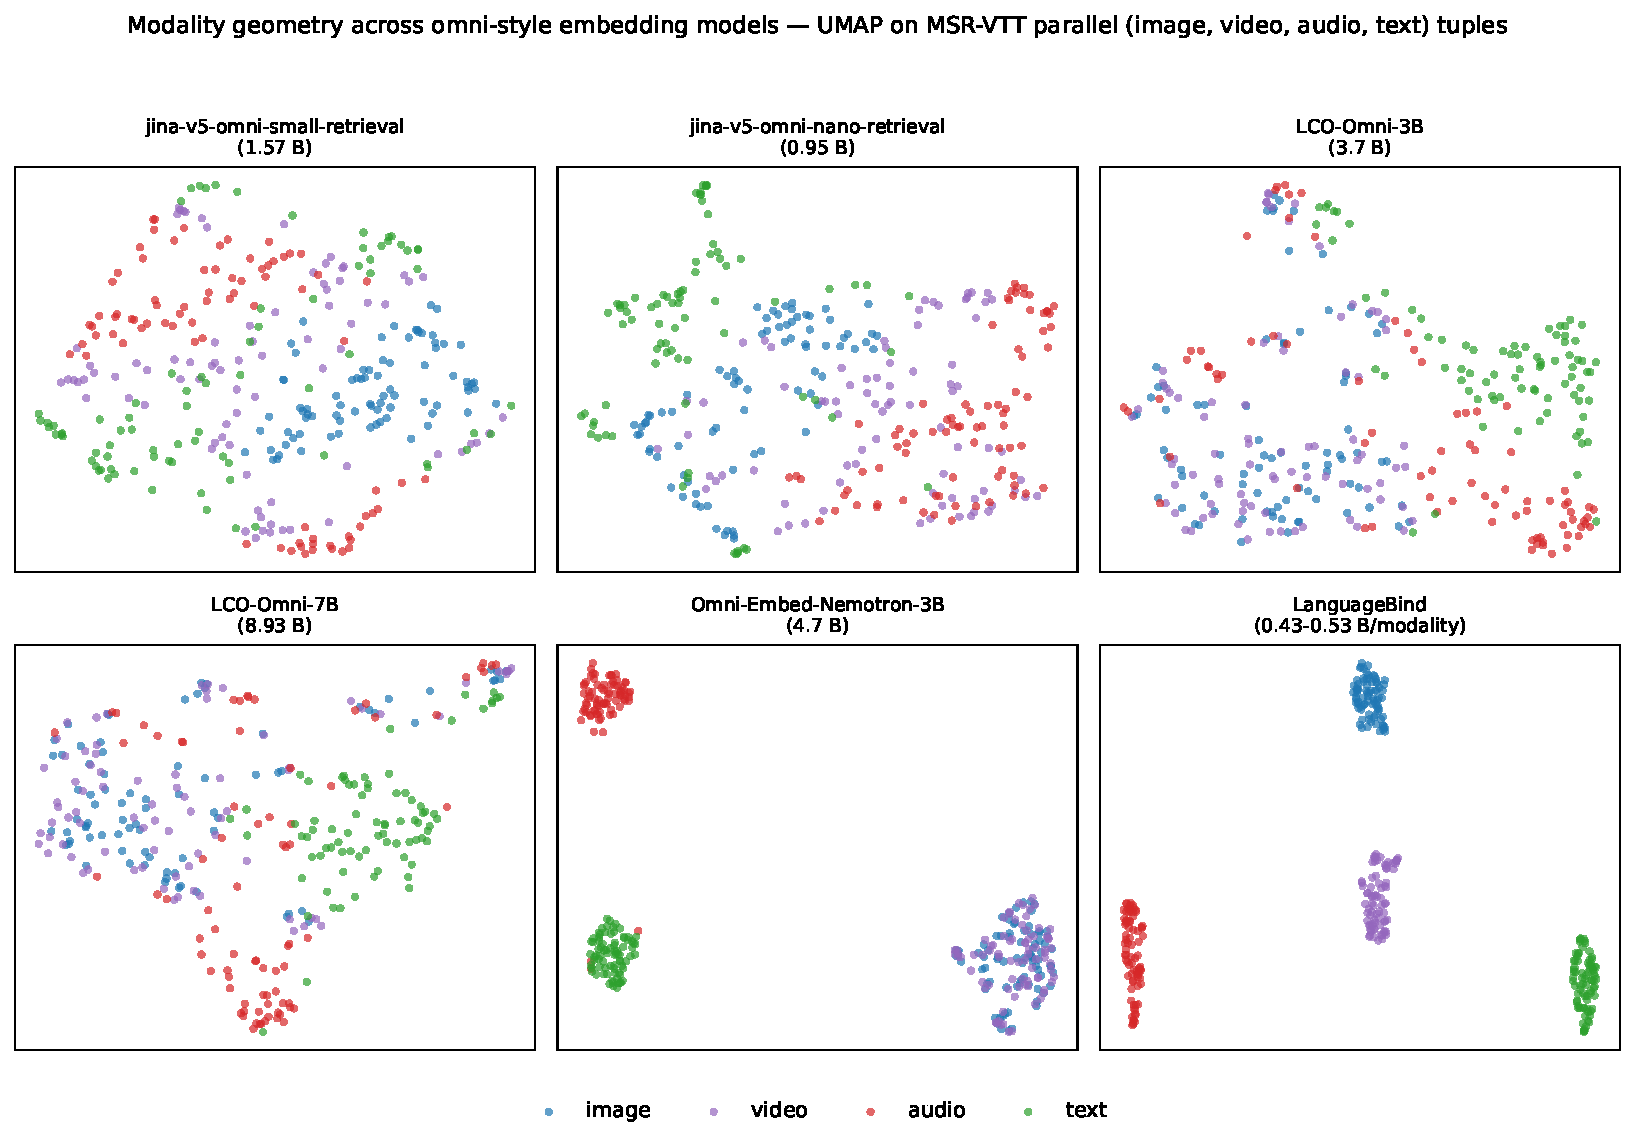
\includegraphics[width=\textwidth]{figures/modality_umap.pdf}
  \caption{2D UMAP of embeddings on $80$ parallel MSR-VTT clips per model.
  Each row of source data contributes four embeddings (image: middle frame; video: full clip; audio: extracted track; text: caption); colours mark modalities.
  UMAP is fit per model on its own $320$ ($80\times4$) points (\texttt{cosine} metric, \texttt{n\_neighbors}=$15$, \texttt{min\_dist}=$0.1$, \texttt{random\_state}=$42$).
  \texttt{LanguageBind}'s frozen per-modality towers produce the canonical modality-gap pattern; the unified-decoder omni models, including the frozen-tower \omniSmall{} and \omniNano{}, produce interleaved geometry.}
  \Description{Six-panel UMAP grid comparing modality clustering across omni embedding models.}
  \label{fig:modality-umap}
\end{figure*}

\paragraph{Image--text.}
The LCO-Embedding family leads on MS-COCO Karpathy: \texttt{LCO-Omni-7B} ($8.93$B) at image$\rightarrow$text R@$1 = 74.0\%$ / text$\rightarrow$image $63.6\%$, \texttt{LCO-Omni-3B} ($3.7$B) at $71.6\%$ / $58.0\%$ (Table~\ref{tab:modality-geometry}).
Our \omniSmall{} variant ($1.57$B, frozen-tower) sits in third place at $68.0\%$ / $57.0\%$, statistically indistinguishable from \texttt{LCO-Omni-3B} on text$\rightarrow$image at the edge of significance, trailing it by $3.6\%$ on image$\rightarrow$text and trailing \texttt{LCO-Omni-7B} by $6$--$7\%$ in both directions; paired-bootstrap $95\%$ confidence intervals are tabulated in the Table~\ref{tab:modality-geometry} footnote.
At $18\%$ the parameter count of \texttt{LCO-Omni-7B} and $42\%$ of \texttt{LCO-Omni-3B}, the frozen-tower design closes most of the omni gap in both directions.
The \omniNano{} variant ($0.95$B) trails the leaders at $36.6\%$ / $27.7\%$, and \texttt{Omni-Embed-Nemo\-tron-3B} ($4.7$B, co-trained) collapses to $23.1\%$ / $1.4\%$. The low score for \texttt{Omni-Embed-Nemotron-3B} is evidence that parameter count alone does not determine outcome on this axis.

\paragraph{Audio--text.}
The LCO-Embedding family leads for this modality as well: \texttt{LCO-Omni-7B} at $27.5\%$ / $29.8\%$, \texttt{LCO-Omni-3B} at $24.5\%$ / $28.5\%$ (Table~\ref{tab:modality-geometry}).
Our \omniSmall{} variant reaches $16.3\%$ / $15.2\%$, trailing \texttt{LCO-Omni-7B} by $11$--$15\%$ and \texttt{LCO-Omni\allowbreak -3B} by $8$--$13\%$; the \omniNano{} variant lands a further $2\%$ below.
\texttt{Omni-Embed-Nemotron-3B} again underperforms at $10.1$ / $9.6\%$ despite being the second-largest model in the table.
Critically, the gap between the \omniSmall{} variant and \texttt{LCO-Omni-7B} is markedly larger on the audio pair ($\sim$$11$--$15\%$ absolute) than on the image pair ($\sim$$6$--$7\%$), under conditions where the centroid distance and paired cosines are within range across all five rows, suggesting the audio bridge into the text-aligned subspace is the weaker of the two projector paths.

\paragraph{Embedding-space geometry across all four modalities.}
Figure~\ref{fig:modality-umap} adds a complementary visual view: a 2D UMAP of $80$ parallel MSR-VTT clips (extracted middle frame, full clip, audio track, and caption), encoded by each model in its natural retrieval protocol.
Three qualitatively distinct patterns appear.
\texttt{LanguageBind} -- the fourth omni-style baseline of Table~\ref{tab:benchmark-summary}, with separate per-modality CLIP-style towers bound to a shared text encoder -- shows the canonical modality-gap pattern from~\cite{modality-gap}: Each modality collapses into a tight, disjoint cluster, with sharp boundaries between them.
\texttt{Omni-Embed-Nemotron-3B} is intermediate. Text is visibly separated from the three other modalities, which themselves overlap somewhat.
The unified-decoder LCO-Omni models and our two frozen-tower \omniSmall{} and \omniNano{} variants produce broadly interleaved geometry: image, video, audio, and text co-mingle in the same neighborhood with substantial overlap, consistent with a single shared embedding space across all four input types rather than four pre-aligned cones.
This geometric picture explains the retrieval-margin behavior reported in the table: Well-mixed clusters have a smaller average modality-cluster offset (lower centroid distance), but their paired-pair coupling also has to compete with same-modality distractions, which is part of why the within-modality R@$1$ gaps remain visible.

\begin{table*}[t]
  \caption{Main benchmark results.
  Bold numeric cells mark the row winner among \omniNano{}, \omniSmall{}, and the strongest open-weight baseline model; bold row labels are benchmark or slice aggregates, and indented rows are task-type averages.
  The ``Strongest open-weight baseline'' column is an orientation point, not a unified controlled ladder.}
  \label{tab:benchmark-summary}
  \centering
  \small
  \setlength{\tabcolsep}{2pt}
  \begin{tabular}{@{}L{0.255\textwidth}rccL{0.245\textwidth}cc@{}}
    \toprule
    Benchmark / task type & \#Tasks & Nano (0.95\,B) & Small (1.57\,B) & Strongest open-weight baseline & Params (B) & Score \\
    \midrule
    \textbf{MIEB Light (Image)} & 51  & 44.24 & 55.01 & LCO-Embedding-Omni-3B & 4.07 & \textbf{61.63} \\
    \quad Image classification & 15 & 44.12 & \textbf{64.12} & LCO-Embedding-Omni-3B & 4.07 & 59.07 \\
    \quad Compositional / vision QA & 11 & 38.85 & 47.61 & LCO-Embedding-Omni-3B & 4.07 & \textbf{52.00} \\
    \quad Image clustering & 2 & 60.46 & \textbf{83.18} & LCO-Embedding-Omni-3B & 4.07 & 73.19 \\
    \quad Visual STS & 4 & 65.92 & \textbf{74.25} & royokong/e5-v & 8.36 & 63.73 \\
    \quad Retrieval & 13 & 25.95 & 31.63 & LCO-Embedding-Omni-3B & 4.07 & \textbf{83.44} \\
    \quad Document retrieval & 6 & 74.21 & \textbf{74.25} & LCO-Embedding-Omni-3B & 4.07 & 72.99 \\
    \midrule
    \textbf{MIEB (Image)} & 125 & 47.87 & 58.00 & siglip-so400m-patch14-384 & 0.88 & \textbf{60.69} \\
    \quad Image classification & 45 & 53.26 & \textbf{68.99} & LCO-Embedding-Omni-3B & 4.07 & 64.30 \\
    \quad Compositional / vision QA & 13 & 40.18 & 49.48 & LCO-Embedding-Omni-3B & 4.07 & \textbf{53.40} \\
    \quad Image clustering & 5 & 72.28 & \textbf{86.01} & LCO-Embedding-Omni-3B & 4.07 & 83.24 \\
    \quad Visual STS & 7 & 75.92 & \textbf{81.74} & LCO-Embedding-Omni-3B & 4.07 & 79.62 \\
    \quad Retrieval & 45 & 30.66 & 37.95 & LCO-Embedding-Omni-3B & 4.07 & \textbf{46.29} \\
    \quad Document retrieval & 10 & 79.25 & 79.25 & Omni-Embed-Nemotron-3B & 4.70 & \textbf{85.64} \\
    \midrule
    \textbf{MIEB Multilingual only (Image)} & 5 & 48.19 & 63.75 & LCO-Embedding-Omni-3B & 4.07 & \textbf{69.04} \\
    \quad Visual STS & 2 & 53.95 & 65.12 & LCO-Embedding-Omni-3B & 4.07 & \textbf{79.62} \\
    \quad Retrieval & 3 & 44.35 & \textbf{62.83} & LCO-Embedding-Omni-3B & 4.07 & 61.99 \\
    \midrule
    \textbf{MMEB-Video (Video)} & 18  & 29.73 & 39.83 & Qwen3-VL-Embedding-8B & 8.14 & \textbf{67.15} \\
    \quad V-CLS (classification) & 5 & 27.85 & 42.73 & Qwen3-VL-Embedding-8B & 8.14 & \textbf{78.39} \\
    \quad V-QA (question answering) & 5 & 39.03 & 44.52 & WeMM-Embedding-8B & 8.77 & \textbf{71.66} \\
    \quad V-RET (retrieval) & 5 & 14.33 & 27.82 & Qwen3-VL-Embedding-8B & 8.14 & \textbf{58.73} \\
    \quad V-MRET (moment retrieval) & 3 & 43.02 & 47.20 & Qwen3-VL-Embedding-8B & 8.14 & \textbf{56.09} \\
    \midrule
    \textbf{MAEB (Audio)} & 30 & 49.69 & 49.96 & LCO-Embedding-Omni-7B & 8.93 & \textbf{52.37} \\
    \quad Retrieval / reranking & 10 & 53.35 & 53.22 & LCO-Embedding-Omni-7B & 8.93 & \textbf{61.67} \\
    \quad Classification / zero-shot & 14 & 53.04 & \textbf{53.71} & LCO-Embedding-Omni-7B & 8.93 & 53.39 \\
    \quad Text matching & 3 & 65.56 & 65.38 & LCO-Embedding-Omni-7B & 8.93 & \textbf{67.30} \\
    \quad Clustering & 3 & 5.96 & 6.13 & clap-htsat-fused & 0.15 & \textbf{22.74} \\
    \bottomrule
  \end{tabular}
  \\[0.4em]
  {\footnotesize MIEB rows use the current MTEB benchmark task composition (MIEB Light 51 tasks, MIEB full 125 tasks, MIEB Multilingual-only 5 tasks). MMEB-Video uses the full $18$-task suite, including MomentSeeker.}
\end{table*}

\begin{figure}[t]
  \centering
  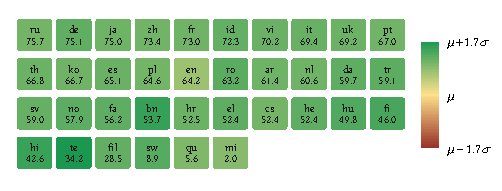
\includegraphics[width=\columnwidth]{figures/multilingual_language_winners.pdf}
  \caption{XM3600 image-language comparison.
  Tiles show \texttt{jina-v5-omni-small}; color is deviation from a five-model language mean.}
  \Description{XM3600 language tiles for jina-v5-omni-small compared with Nano, LanguageBind, LCO-3B, and Nem-3B; LCO-7B is discussed by aggregate score.}
  \label{fig:multilingual-comparison}
\end{figure}

\begin{figure}[t]
  \centering
  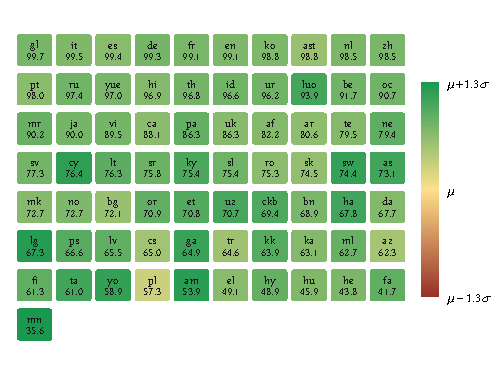
\includegraphics[width=\columnwidth]{figures/audio_language_averages.pdf}
  \caption{Per-language audio retrieval.
  Tiles show \texttt{jina-v5-omni-small} on shared CommonVoiceMini21/FLEURS languages; color is deviation from the mean of the baseline models.}
  \Description{Audio language tiles for jina-v5-omni-small compared with Nano, LCO-3B, Nem-3B, and LanguageBind Audio across the shared CommonVoiceMini21/FLEURS languages.}
  \label{fig:audio-language-comparison}
\end{figure}
